%%
%% This is file `example/ch_intro.tex',
%% generated with the docstrip utility.
%%
%% The original source files were:
%%
%% install/buptgraduatethesis.dtx  (with options: `ch-intro')
%% 
%% This file is a part of the example of BUPTGraduateThesis.
%% 

\chapter{基于动态阈值的成对注意力机制模型}
\label{chapter:3}
本章主要提出了一种基于动态阈值的成对注意力机制模型。首先章节~\ref{sec:dpam_intro}描述了算法的研究背景;接着,在章节~\ref{sec:dpam_algori}中介绍了基于动态阈值的成对注意力机制模型结构,包括算法的设计、模型的学习与预测等过程;章节~\ref{sec:dpam_exper}中介绍实验设置相关内容,对实验数据集,对比方法等进行介绍;章节~\ref{sec:dpam_exper_result}对实验结果进行分析,章节\ref{sec:dpam_analysis}对实验结果进行进一步的分析和讨论,章节\ref{sec:dpam_conclu}对本章内容进行总结。

\section{引言}
\label{sec:dpam_intro}

在司法领域,基于严格定义的司法法条进行犯罪分类是一项非常繁杂的工作。法官通常需要阅读若干类似的案例,针对事实描述给定涉及的法条,这件事是非常耗时并且需要专业知识的。通常来讲,这个任务被当作多标签分类分体,用于提高工作效率和节省人力成本。在本课题中,采用多标签分类处理这个问题,帮助法官快速准确的针对案情描述挑选出合适的法条。

然而,这个问题是非常困难的,面临两个主要问题。一个问题是大多数案情描述涉及的法条数量是不确定的,称为标签动态问题。通过在大规模数据上对70个法条进行分析,案列包含的标签数量有很大差异,其结果如图~\ref{fig:dis1}所示:
\begin{figure*}[htb]
\centering
% 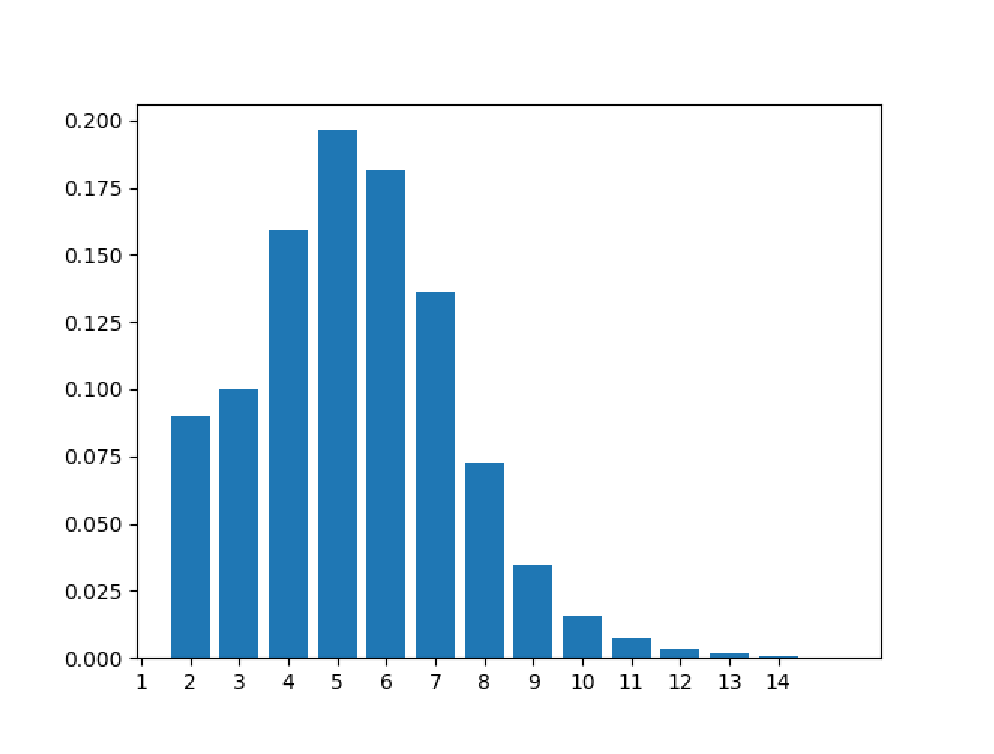
\includegraphics[scale=0.5,clip=true]{1.eps}
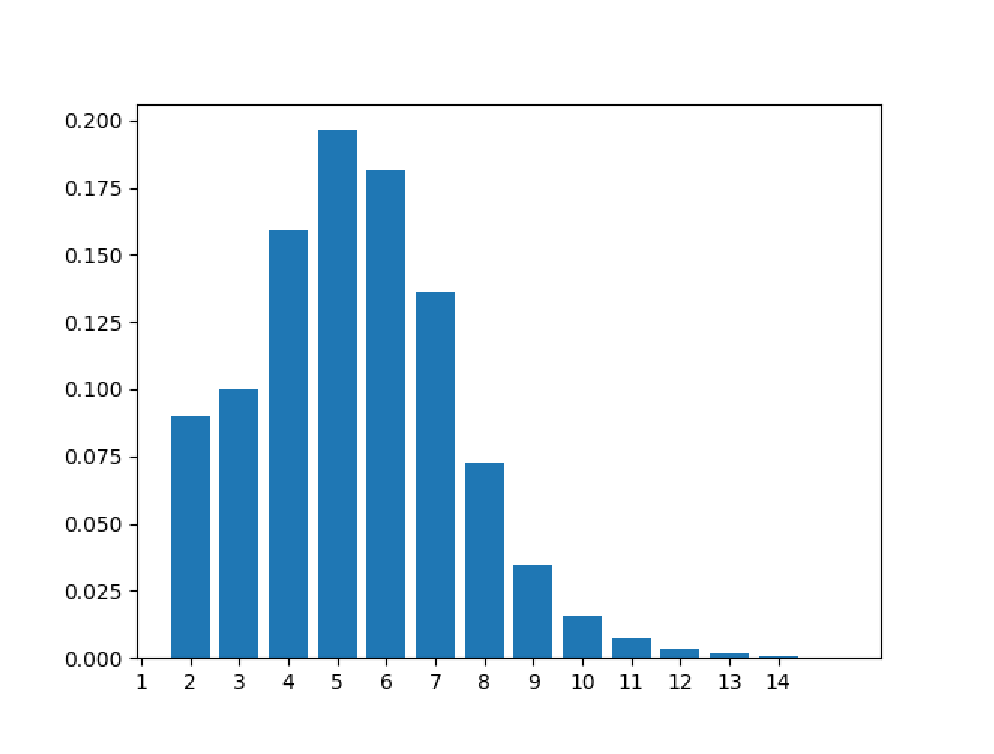
\includegraphics[scale=0.5, viewport=0 0 450 350,clip=true]{./sources/dpam_statistic1.eps}
\caption{\label{fig:dis1}样本平均标签个数分布统计图}
\end{figure*}

从图中可以看出,案情描述对应的法条个数从2到14不等,具有很大的差异性,因此很难通过固定标签个数来进行法条预测。

另一个挑战是标签不均衡问题。如果一个多标签分类数据集上一部分数据的标签数量远远小于另一部分数据,那么这个多标签分类数据集被认为是不均衡的。针对同一份案例数据进行分析,其结果如图~\ref{fig:tail}所示,其中,x轴代表法条集合大小,y轴代表样本比例占比。

\begin{figure*}[htb]
\centering
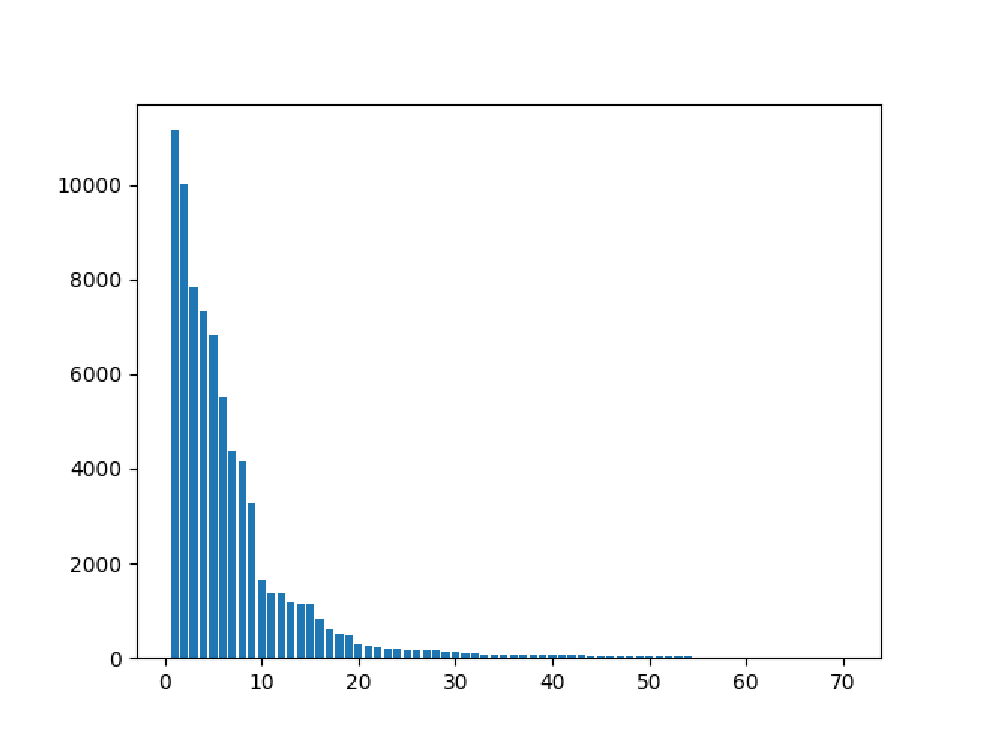
\includegraphics[scale=0.5,clip=true]{./sources/dpam_statistic2.eps}
\caption{\label{fig:tail}样本标签出现次数统计图}
其中,x代表按出现频次排序的标签,y代表标签出现的次数。
\end{figure*}


从图中可以看出,每种法条出现的数量符合长尾分布,这意味着很多法条很少在审判中被引用。大多数传统的多标签分类算法在训练过程中通过最小化整体分类误差来进行优化,这种方式假设所有标签拥有同等的重要性。这种假设使得分类算法在训练过程中偏向于向数量占比多的标签进行学习。虽然法条定义可以体现不同法条之间的一些相关信息用于缓解标签不均衡问题(例如表~\ref{t:relevant_article}所示,刑法第一百九十七条和刑法第一百九十一条是非常相似的。),但是目前在判决预测研究中没有工作考虑这方面的问题。
\begin{table}[htb]
    \caption{法条定义中相关法条}
    \label{t:relevant_article}
    \centering
    \begin{tabular}{lp{12cm}p{8cm}}
    \hline
    &\emph{\textbf{刑法第一百九十七条}: 使用伪造、变造的国库券或者国家发行的其他有价证券,进行\emph{\textbf{诈骗}}活动,数额较大的,处五年以下有期徒刑或者拘役... \newline
    \textbf{刑法第一百九十一条}: 明知是毒品犯罪、黑社会性质的组织犯罪、恐怖活动犯罪、走私犯罪、贪污贿赂犯罪、破坏金融管理秩序犯罪、\emph{\textbf{金融诈骗}}犯罪的所得及其产生的收益,为掩饰、隐瞒其来源和性质,有下列行为之一的,没收实施以上犯罪的所得及其产生的收益...}\\
    \hline
    \end{tabular}
\end{table}



现有的很多多标签分类工作都引入了标签之间的关联信息,然而,这些工作都将多标签分类和阈值预测器分开学习,并且忽略了标签不均衡问题。为了处理这个问题,本课题提出了一种多任务学习框架用于联合学习多标签分类模型(简称\textbf{DPAM})和阈值预测器。针对第二个问题,本课题采用法条描述信息来建模标签之间的成对关系,并针对标签集合构造软注意力机制矩阵,最后通过设计一个多任务学习框架联合学习这两个任务,利用任务间的交互关系,提高模型泛化性能。

总体来讲,本章工作的主要贡献如下:
\begin{itemize}
    \item 本课题首次在司法领域对案情描述和法条定义进行探索用于判决预测。
    \item 本课题设计了一种多标签分类结构用于联合学习多标签分类器和阈值预测器,通过这种方式,DPAM可以通过利用相关任务包含的信息防止模型的过拟合,提高模型的泛化性能。
    \item 一种基于法条定义的成对注意力模型被引用分类模型中,用于缓解标签不均衡问题。
    \item 通过在两个真实数据集上的扩展实验,与基线模型进行对比,对本课题提出的DPAM模型进行验证。
\end{itemize}

\section{DPAM算法设计}
\label{sec:dpam_algori}

在本节中,本课题详细介绍提出的动态成对注意力机制模型。如图~\ref{fig:model}所示是\textbf{DPAM}模型架构图。具体来讲,本模型包含两部分:一个成对注意力机制模型(简称\textbf{PAM})用于得到标签关联得分,一个动态阈值预测器得到参考阈值用于决定标签和给定案情描述是否相关。最后,采用多任务学习方法联合学习这两个任务。

\begin{figure*}[htb]
\centering
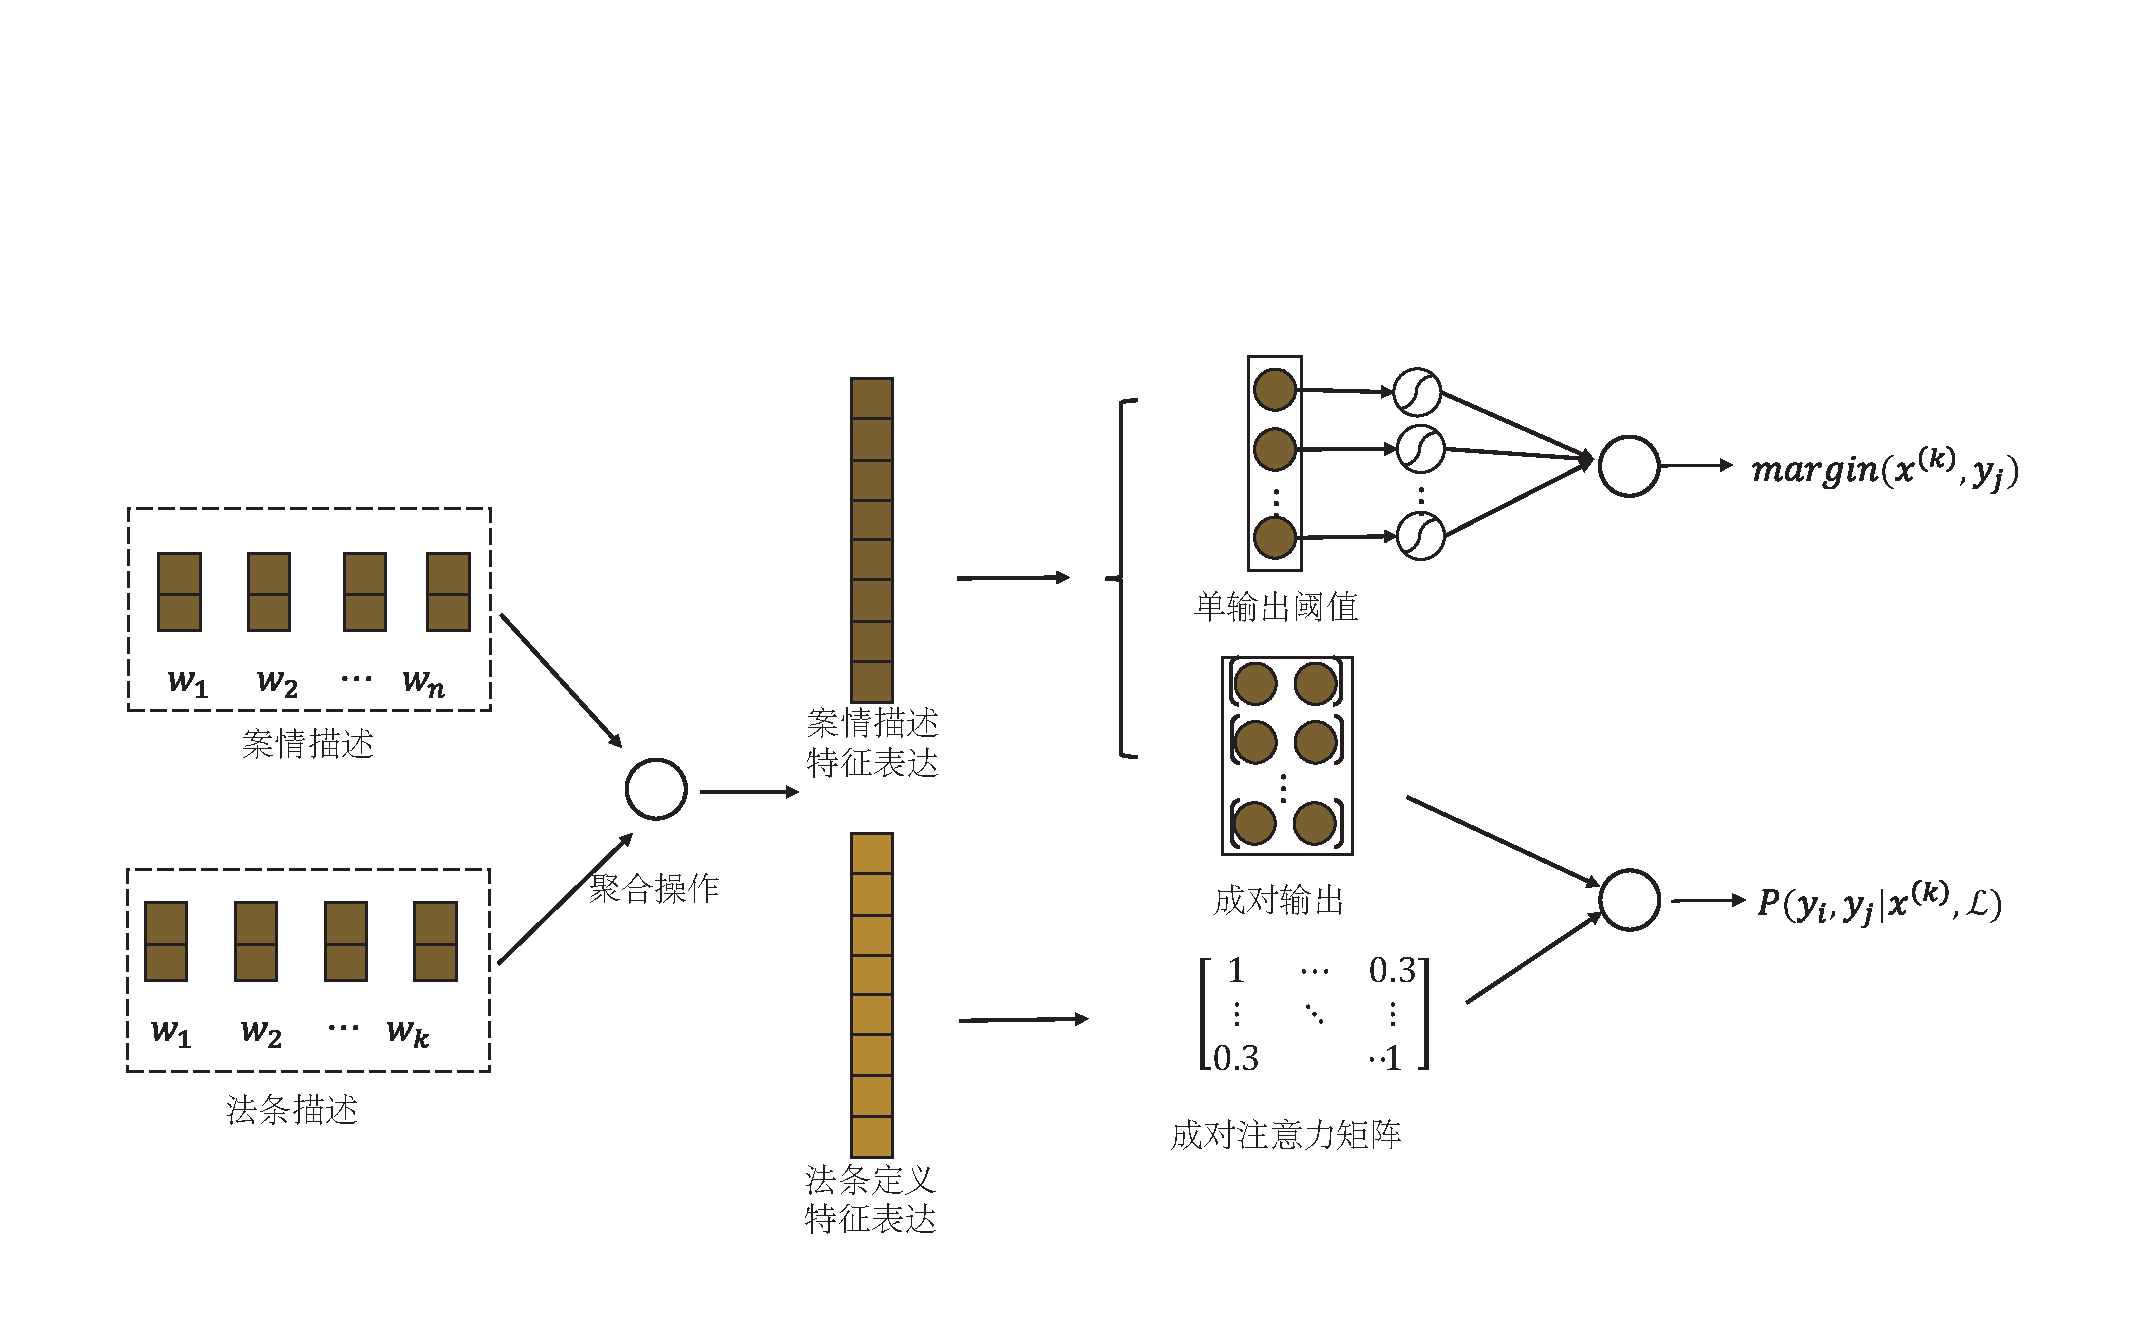
\includegraphics[scale=0.48,viewport=45 50 980 500,clip=true]{./sources/dpam_DPAM.eps}
\vspace{-10pt}
\caption{\label{fig:model} 动态成对注意力机制模型结构图 }
\vspace{-5pt}
\end{figure*}


\subsection{成对注意力机制模型}
在司法领域,每个案情描述都由一个集合的词组成。本课题采用词袋表示作为输入,并将每个词映射带一个连续的向量空间。之后本课题将所有的词向量进行聚合组成案情表达和标签描述表达。PAM将标签之间的关联进行考虑。具体来讲,针对每一个训练样本$(x^{(k)}, Y^{(k)})$,PAM枚举标签集合$Y^{(k)}$中的成对关系,利用这种关系,本模型可以引入标签关联信息。以$Y^{(k)}=\{y_1,y_2,y_3\}$举例,枚举之后,原始标签集合变为 $\{(y_1,y_2),(y_1,y_3),(y_2,y_3)\}$。

更正式地,用$\textbf{V}^I=\{\vec{v}^I_j\in \mathbb{R}^{D_v}|j=1,\dots,N\}$表示在一个$D_v$维连续空间中的所有词向量。针对每个案情描述和标签定义,本模型采用如下方式将词向量聚合为案情表达和标签描述表达:

\begin{equation}
    \begin{aligned}
        \vec{v}^{(e,k)}&=g(\vec{v}^I_j:j\in x^{(k)})\\
        \vec{v}^{(l,i)}&=g(\vec{v}^I_j:j\in l^{(i)})\\
    \end{aligned}
\end{equation}

其中,$g(\cdot)$代表聚合函数。在本课题的工作中,使用TextCNN~\cite{Kim14}用于构造输入向量。给定案情描述$x^{(k)}$和标签定义$\mathcal{L}$,PAM考虑成对$(y_i,y_j)\in Y^{(k)}$条件概率计算公式如下:

\begin{equation}
    P(y_i,y_j|x^{(k)},\mathcal{L})=P(y_i,y_j|x^{(k)})P(l^{(i)},l^{(j)})
\end{equation}
其中,$P(y_i,y_j|x^{(k)})$ 和 $P(l^{(i)},l^{(j)})$ 分别进行计算。

为了解决标签不均衡问题,本课题引入成对标签关联信息。众所周知,注意力模型在传统的序列建模,例如LSTM和GRU,采用软加权机制对子序列进行加权。为了提高稀疏成对标签的重要性,本课题将传统的注意力机制扩展到成对关系集合中,称为成对注意力机制。给定标签描述表达$\vec{v}^{(l,i)}$ 和 $\vec{v}^{(l,j)}$,成对注意力矩阵计算如下:

\begin{equation}\label{eq:similiar}
P(l^{(i)},l^{(j)})=\frac{\vec{v}^{(l,i)}\cdot\vec{v}^{(l,j)}}{\sum_{j=1,j\neq i}^{|C|}\vec{v}^{(l,i)}\cdot\vec{v}^{(l,j)}}
\end{equation}

在本模型中,$P(l^{(i)}, l^{(j)})$可以被看做标签集合$Y^{(k)}$中的标签对$(y_i, y_j)$的注意力机制得分。这种机制使得不在样本标签集合中的标签同样影响最后的损失函数,并能增强具有类似描述信息的稀疏成对标签的重要性,这样我们就可以缓解标签不平衡问题。

因此,训练数据中成对标签的后验概率$P(y_i,y_j|x^{(k)})$由softmax函数计算如下:
\begin{displaymath}
P(y_i,y_j|x^{(k)})=\frac{exp(\vec{v}^{(e,k)}\textbf{W}\vec{y}^{(i,j)})}{\sum_{\vec{y}^{(i,j)}\in\mathbb{Y}}exp(\vec{v}^{(e,k)}\textbf{W}\vec{y}^{(i,j)})}
\end{displaymath}

其中$\textbf{W}=\mathbb{R}^{D_V\times |C|}$是交互矩阵,$\vec{y}^{(i,j)}$是$|C|$大小的向量,并且$\vec{y}^{(i,j)}$ 中共现标签位置为1,其他位置为0。$\mathbb{Y}$是考虑不同标签对$(y_i,y_j)$的所有可能向量。将PAM的目标函数定义为所有案情的对数似然函数,其定义如下:

\begin{eqnarray}\label{eq:pam}
l_{pam}&=&\sum_{x^{(k)}\in X}\sum_{(y_i,y_j)\in E(Y^{(k)})}\log P(y_i,y_j|x^{(k)},\mathcal{L})\\\nonumber
&=&\sum_{x^{(k)}\in X}\sum_{(y_i,y_j)\in E(Y^{(k)})}\Big(\log P(y_i,y_j|x^{(k)})+\log P(l_i,l_j)\Big)
\end{eqnarray}

其中$ E(Y^{(k)})$代表$Y^{(k)}$中成对枚举关系。

最后,PAM基于学习到的参数$\textbf{W}$输出针对新实例$x^{(k)}$每个标签$y_i$的概率:
$$
P(y_i|x^{(k)})=\frac{exp(\vec{v}^{(e,k)}\textbf{W}_{*i})}{\sum_{i=1}^{|C|}exp(\vec{v}^{(e,k)}\textbf{W}_{*i})}
$$

其中,$\textbf{W}_{*i}$代表$\textbf{W}$的第$i$列。

\subsection{动态阈值预测器}
通过PAM,每个标签$P(y_i|x^{(k)})$的输出概率通过阈值进行预测最终结果,总的来说,本模型的目标是学习一个决策边界用来决定这个标签是否与给定案情描述相关。直观上来说,如果$P(y_i|x^{(k)})$大于$y_i$的决策边界$t_i$,那么标签$y_i$和$x^{(k)}$相关并且$y_i\in Y^{(k)}$;如果$P(y_i|x^{(k)})$小于$y_i$的决策边界$t_i$,标签$y_i$和$x^{(k)}$不相关。特别低,本模型使用下面的函数针对每个案情给定预测标签的置信度:

\begin{equation}
margin(x^{(k)},y_i)=[P(y_i|x^{(k)})-t_i)]\cdot Seg(x^{(k)},y_i)
\end{equation}
其中 $t_i\in \textbf{T}^{1\times |C|}$ 是针对$y_i$学习到的决策边界. $Seg(x^{(k)},y_i)$ 是一个分割函数,其定义如下:


\begin{displaymath}
Seg(x^{(k)},y_i)=\left\{
\begin{aligned}
1 & , & y_i\in Y^{(k)} \\
-1 &, & y_i\notin Y^{(k)}
\end{aligned}
\right.
\end{displaymath}

在本模型中,$margin(x^{(k)},y_i)$代表标签$y_i$与案情$x^{(k)}$相关的软边界。$margin(x^{(k)},y_i)>0$ 代表$x^{(k)}$被正确分类为$y_i$,$margin(x^{(k)},y_i)<0$代表标签$y_i$和$x^{(k)}$不相关。
之后本模型使用下面的函数决定所有样本案例的每个标签:
\begin{equation}\label{eq:dyn}
l_{dyn}=\sum_{x^{(k)}\in X}\sum_{y_i\in Y^{(k)}}\log\left[1+exp(-margin(x^{(k)},y_i))\right]
\end{equation}

最后,通过结合公式~\ref{eq:pam}和公式~\ref{eq:dyn},本模型定义多任务学习方法如下:
\begin{equation}\label{eq:multi}
\ell=l_{pam}+l_{dyn}-\lambda\left\|\Theta\right\|_2
\end{equation}

其中$\lambda$是正则化系数,$\Theta$是需要学习的模型参数(例如$\Theta=\{\textbf{W}^{D_V\times |C|},\textbf{V}^I,\textbf{T}^{1\times|C|}\}$)。

\subsection{模型学习与预测}
为了学习DPAM模型的参数,本模型采用随机梯度下降进行算法学习。每次迭代,通过公式\ref{eq:multi}更新参数。然而,直接通过公式\ref{eq:pam}优化由于与$2^{|C|}$成正比的高计算复杂度是非常困难的。因此,本模型采用负采样技术\cite{mikolov2013}进行模型优化,新的目标函数定义如下:
\begin{displaymath}
\begin{aligned}
\ell_{NEG} &= \sum_{x^{(k)}\in X}\sum_{(y_i,y_j)\in E(Y^{(k)})}\Big( \log\sigma(\vec{v}^{(e,k)}\textbf{W}\vec{y}^{(i,j)})\\
&+n_{neg}\cdot \mathbb{E}_{\vec{y}^{neg}\sim P_{\mathcal{Y}}}[\log\sigma(-\vec{v}^{(i)\top}\textbf{W}\vec{y}^{neg})]+\log P(l^{(i)},l^{(j)})\Big)\\
\end{aligned}
\end{displaymath}

其中,$\sigma(x)$是sigmoid函数$\sigma(x)=\frac{1}{(1+e^{-x})}$,$n_{neg}$ 是负样本个数,$\vec{y}^{neg}$是采样向量,它通过所有成对标签组合的经验分布得到。可以看出,带有负采样的DPAM模型的目标是增加给定案情的正标签对组合的概率,减少负样本对组合的高铝。之后采用随机梯度下降算法来最大化新的目标函数来进行模型学习。

在训练阶段,本课题发现模型性能的提升不明显。分析得出其原因是由于注意力机制矩阵是由聚合后的词表达进行初始化的。因此在开始的迭代轮次中,注意力机制矩阵变成了模型的噪声。为了获得更好的性能,本课题设计了一种新的学习策略:对前1000次迭代,设置$P(l^{(i)},l^{(j)})=1$,在初始阶段之后,假定已经获得了稳定的词向量表达,之后再通过公式\ref{eq:similiar}在每次迭代中计算注意力机制矩阵。算法学习的细节如流程图\ref{alg:algo}所示:

\begin{algorithm}[htbp]
\caption{联合训练模型框架}
\label{alg:algo}
\begin{algorithmic}[1]
% \Require
% The set of positive samples for current batch, $P_n$;
% The set of unlabeled samples for current batch, $U_n$;
% Ensemble of classifiers on former batches, $E_{n-1}$;
% \Ensure
% Ensemble of classifiers on the current batch, $E_n$;
\State 随机初始化模型参数 $\Theta=\{\textbf{W}^{D_V\times |C|},\textbf{V}^I,\textbf{T}^{1\times|C|}$\}
\label{code:fram:initialize parameters}
\State iter = 0
\label{code:fram:begin}
\State 设置 $n_{burn} = 1000$
\label{code:fram:setvalue}
\Repeat
\label{code:fram:repeat}
\State $iter \leftarrow iter+1$
\label{code:fram:re_value}
\If {$iter < n_{burn}$}
\label{code:fram:if1}
\State 设置 $P(l^{(i)},l^{(j)}) = 1$
\label{code:fram:init1}
\For{$i = 1,...,|X|$}
\label{code:fram:for1}
\State 针对实例 $x^{(k)}$
\label{code:fram:task_join1}
\State 通过公式(\ref{eq:multi})计算梯度$\nabla(\theta)$ 
\label{code:fram:com_grad}
\State 更新模型$\theta \leftarrow \theta + \epsilon \nabla(\theta)$
\label{code:fram:update_grad}
\EndFor
\Else
\label{code:fram:else1}
\State 通过公式(\ref{eq:similiar})计算$P(l^{(i)},l^{(j)})$
\label{code:fram:com_Sim}
\EndIf
\Until{(收敛 或者 $t > num$)}
\State
\Return $\{\textbf{W}^{D_V\times |C|},\textbf{V}^I,\textbf{T}^{1\times|C|}\}$;
\end{algorithmic}
\end{algorithm}

利用学到的参数,判决预测策略如下。针对案情$x^{(k)}$,标签集合由标签得分是否大于标签阈值决定。预测过程如下:
\begin{eqnarray}\label{eq:pred}
s(Y^{(k)}|x^{(k)}) &=& \sum_{y_i\in Y^{(k)}}I\Big(\frac{exp(\vec{v}^{(e,k)}\textbf{W}_{*i})}{\sum_{i=1}^{|C|}exp(\vec{v}^{(e,k)}\textbf{W}_{*i})}>t_i\Big)
\label{eq:prediction}
\end{eqnarray}

其中,$I(\cdot)$代表索引函数,$s(Y^{(k)}|x^{(k)})$是针对案情$x^{(k)}$,标签集合$Y^{(k)}$中标签的得分。通过公式\ref{eq:pred},针对输入的案情描述,根据前向过程计算每个标签的得分,选取得分大于阈值的作为预测结果。

\section{实验设置}
\label{sec:dpam_exper}

在本节中,主要介绍本模型的实验设置,首先介绍实验所使用的数据集,之后介绍对比的基线模型以及实验参数的设置情况。

\subsection{数据集介绍}
本课题在两个真实数据集上进行实验验证,数据来源于裁判文书网\footnote{http://wenshu.court.gov.cn/Index}。裁判文书网是由中华人民共和国政府开放的网站。它记录了中国超过3000个法院的裁判文书。在本研究中,本课题收集了2014年到2016年的40256个案由是诈骗和其他少量混合罪名相关的裁判文书。

本课题首先对这些数据进行预处理。本课题删除了一些无效数据,之后从剩余的裁判文书中抽取所有的标签集合和案情描述。经过数据预处理,本课题得到包含70个法条标签的17160个诈骗案由样本数据的数据集,以及包含30个法条标签的4033个混合案由样本数据的数据集。数据分析如表~\ref{t:statistic}所示。最后,本课题将数据以8比2将数据划分为训练集和测试机两部分。
\begin{table*}[htb]
\centering
\caption{实验所用两个司法数据集信息统计表}
\label{t:statistic}
\begin{tabular}{cccccc}
\hline
\multirow{2}{*}{数据集} & \multirow{2}{*}{样本个数} & \multirow{2}{*}{标签个数} & \multirow{2}{*}{\begin{tabular}[c]{@{}c@{}}平均 \\ 案情长度\end{tabular}} & \multirow{2}{*}{\begin{tabular}[c]{@{}c@{}}平均标签\\ 定义长度\end{tabular}} & \multirow{2}{*}{\begin{tabular}[c]{@{}c@{}}平均样本\\ 标签个数\end{tabular}} \\
& & & & & \\ \hline
诈骗案由数据集 & 17160 & 70 &1455 &136 &4.1 \\
混合案由数据集 & 4033 & 30 &2533 &123 &2.4 \\ \hline
\end{tabular}
\end{table*}

\subsection{模型评估}
本课题通过和以下模型进行实验对比进行实验验证:
\begin{itemize}
    \item \textbf{POP}: 将出现频次最高的K个标签作为测试数据的预测结果(在本模型中,K=5)。
    \item \textbf{BSVM}:一种一阶多标签分类模型\cite{Elisseeff2001A},在这个模型中,每种标签的预测当作一个二分类问题,之后采用SVM作为分类器对每种标签单独进行分类,之后合并每个分类器的结果。
    \item \textbf{ML-KNN}:ML-KNN~\cite{zhang2007ml}是一种常见的一阶多标签分类模型。基于统计的方法针对新的样本,选取与它最近邻的若干个样本的标签作为结果。ML-KNN采用最大先验原理决定标签集合。
    \item \textbf{BP-MLL}:这种方法\cite{zhang2006multilabel}是一种流行的二阶方法。它采用前馈神经网络通过一种新型的成对损失用来进行多标签分类。
    \item \textbf{TextCNN-NLL}:一种二阶多标签分类算法,采用卷积神经网络\cite{Kim14}作为输入,利用与BL-MLL方法一样的损失进行优化。
    \item \textbf{CC}:分类链\cite{ReadPHF11}是一种新型的链式分类算法,它可以在可接受的计算复杂度范围内建模标签关联信息。
\end{itemize}

针对BSVM,ML-KNN,BP-MLL,TEXTCNN-MLL和CC,本课题使用公开的PV模型\cite{le2014distributed}进行案例表示。针对每个模型,本课题在两个数据集上采用维度$k\in \{64,128,192,256,320\}$进行20次重复试验。本课题对实验结果进行平均后与本模型进行对了,实验结果在下面的章节进行分析。

\section{实验结果}
\label{sec:dpam_exper_result}
\subsection{子模型性能验证}
首先,本课题在两个数据集上验证模型的有效性。目的是为了验证分别引入注意力矩阵和动态阈值机制是否有效。为了进行比较,本课题采用相同的参数设置,同样使用320维特征表达进行实验。

\subsubsection{注意力矩阵的性能}
在本节中,本课题研究注意力矩阵的影响。针对本课题的DPAM模型,将动态阈值机制替换为简单的分割点\cite{Tsoumakas2007Random, clare2001knowledge}用来决定给定案例标签集合的大小。本课题将这个模型命名为静态成对注意力机制模型(简称SPAM)。之后进一步忽略通过标签定义学习到的注意力矩阵的影响(例如,针对注意力矩阵中的元素,设置为固定分数),本课题将消减后的模型称为静态成对模型(简称SPM)。表~\ref{tab:comPairWise}展示了这两种方法的性能对比。从结果中可以得到以下结论:(1)SPAM几乎在两个数据集上所有的评价指标上好于SPM,例如,诈骗案由数据集上,Macro-R, Macro-F1和Jaccard的结果分别提升了$1.8\%$, $1.1\%$, 和 $1.3\%$。(2)与SPM比较,SPAM在Macro-P上的提升非常微小。原因是由于SPAM与SPM相比可以预测出更多的正确标签,但是它不能恰当的处理阈值问题。在预测阶段,一些置信度不高的标签仍旧有效,因此在Macro-P上的性能提升并不明显。
\begin{table}[htb]
\caption{\label{tab:comPairWise}SPM和SPAM实验对比表}
\centering
\begin{tabular}{llclll}
\toprule%\end{tabular}
数据集&方法 & Macro-P & Macro-R & Macro-F1 & Jaccard \\
\midrule
\multirow{2}{*}{\begin{tabular}[c]{@{}c@{}}诈骗案由 \\数据集\\ \end{tabular}} & SPM & 0.572& 0.372& 0.430& 0.768 \\
                                                                              & SPAM & 0.574& 0.390& 0.441& 0.781 \\
                                                                              \hline
\multirow{2}{*}{\begin{tabular}[c]{@{}c@{}}混合案由 \\数据集\\ \end{tabular}} & SPM & 0.645& 0.322& 0.424& 0.623 \\
                                                                              & SPAM& 0.649& 0.340& 0.448& 0.626 \\
\bottomrule
\end{tabular}
\end{table}

该表在不同指标上对SPM和SPAM模型在司法分类任务上进行了实验对比,结果显示,SPAM模型相对于SPM模型在Macro-R,Macro-F1,Jaccard指标上性能提升明显。

\subsubsection{动态阈值预测器的性能}
本课题进一步分析了模型中动态阈值预测器的性能。针对本课题的DPA模型,采用消减策略忽略注意力矩阵中的权重,将新模型命名为动态成对模型(简称DPM)。本课题将DPM与几种常见的阈值策略进行比较,例如,分割点策略和线性机制,实验结果展示在表~\ref{tab:comDynamic}中。

\begin{table}[hbt]
\caption{\label{tab:comDynamic}阈值策略对比表}
\centering
\setlength{\tabcolsep}{2pt}
\begin{tabular}{clclll}
\toprule%\end{tabular}
数据集&方法 & Macro-P & Macro-R & Macro-F1 & Jaccard\\
\midrule
\multirow{3}{*}{\begin{tabular}[c]{@{}c@{}}诈骗案由数据集\\ \end{tabular}} &分割点策略 & 0.560& 0.371& 0.425& 0.762 \\
&线性模型 & 0.573& 0.372& 0.428& 0.767 \\
&DPM & 0.604& 0.377& 0.433& 0.772 \\
\hline
\multirow{3}{*}{\begin{tabular}[c]{@{}c@{}}混合案由数据集\\ \end{tabular}} &分割点策略 & 0.513& 0.201& 0.183& 0.438 \\
&线性模型 & 0.393& 0.204& 0.185& 0.435 \\
& DPM & 0.653& 0.329& 0.457& 0.613 \\
\bottomrule
\end{tabular}
\vspace{-10pt}
\end{table}

如表所示是分割点策略,线性模型,DPM模型在司法分类任务上不同评价指标实验结果对比,
从实验结果得到一下结论:(1)线性机制\cite{Zhang2014A,Elisseeff2001A}的结果好于ad-hoc\cite{Brinker2008Multilabel,Tsoumakas2007Random}策略。(2)DPM性能好于线性机制。以诈骗案由数据集为例,在Macro-P,Macro-F1和Jaccard上的结果分别提升了$3.1\%$, $0.5\%$, and $0.5\%$。(3)与线性模型相比,DPM在Macro-R上性能提升并不明显。原因是动态阈值机制重点在于如何学习一个鲁棒的阈值边界来剔除不置信的标签,因此,它在Macro-P上的表现要好于Macro-R。

\subsubsection{子模型性能比较}
在本节中,本课题将SPAM和DPM和DPAM模型进行对比,以便看到两个子模型的差异。图~\ref{fig:comSubm}展示了三个模型的结果比较:
\begin{figure*}[htbp]%[htbp]
\centering
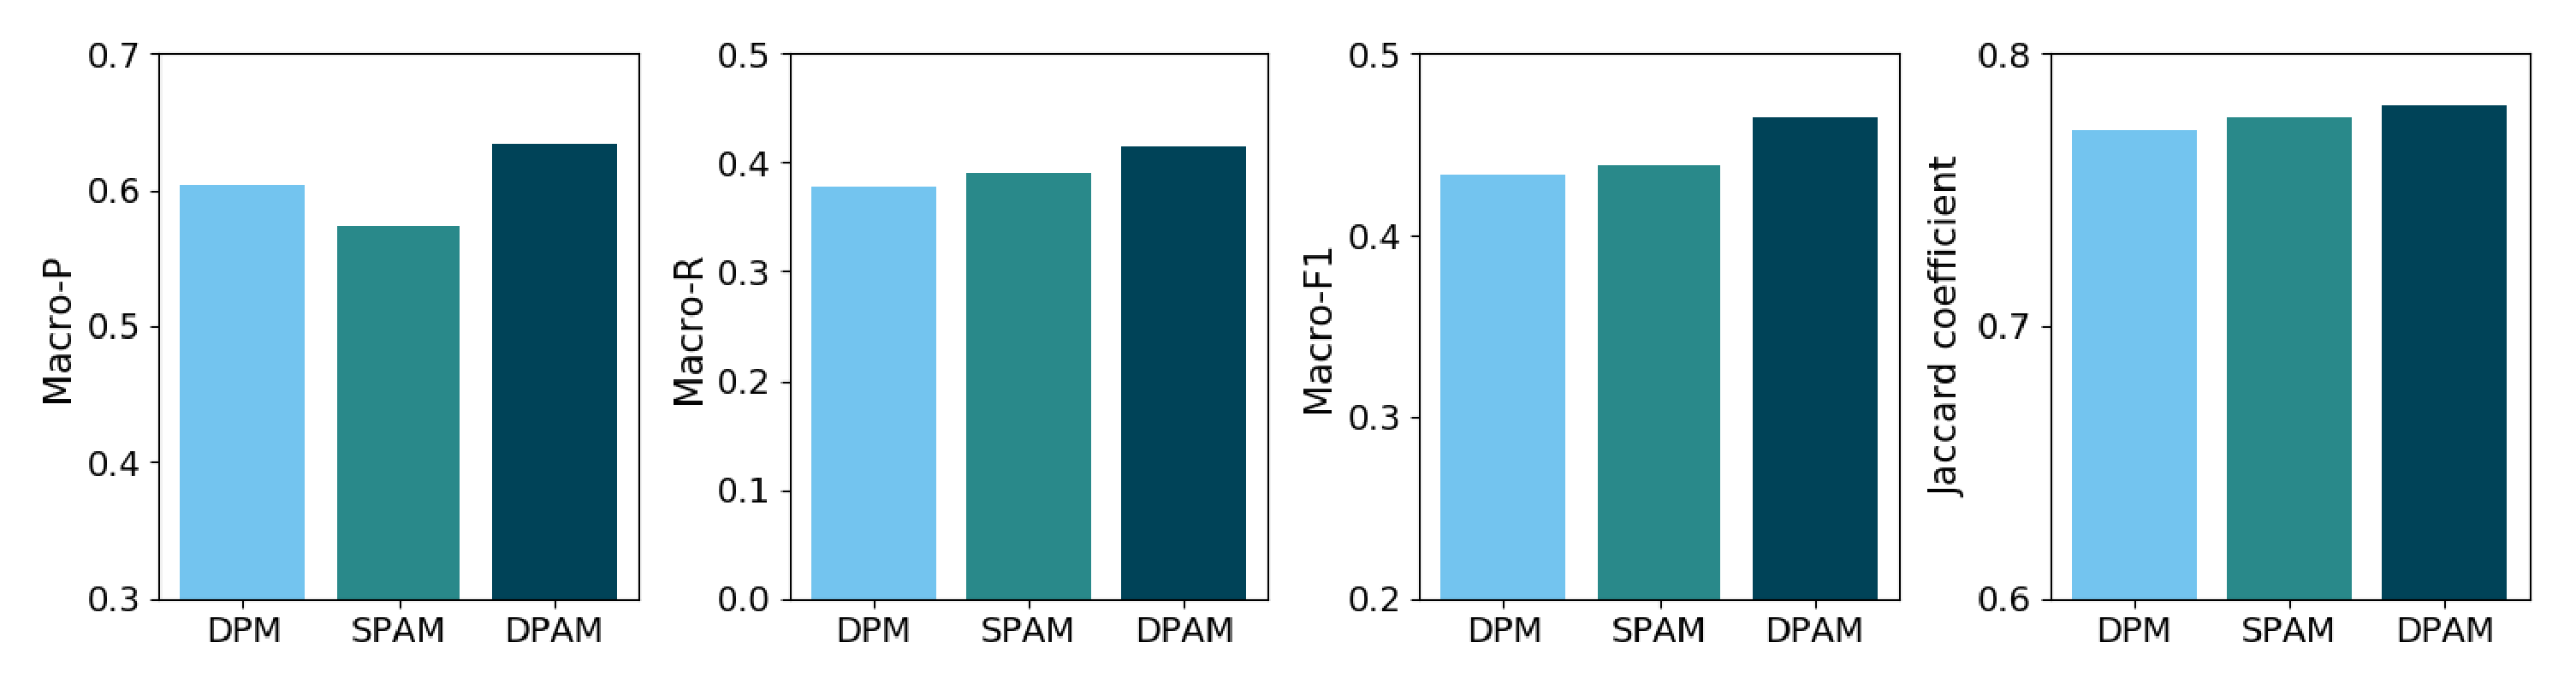
\includegraphics[scale=0.30, clip=true]{./sources/dpam_comSubm2.eps}
\caption{\label{fig:comSubm}DPAM与子模型结果对比图}
\end{figure*}

该图展示了DPAM与DOM,SPAM两个子模型使用Marco-P,Macro-R,Macro-F1作为评价指标在诈骗案由数据集上的实验结果。从实验结果中,可以得到一个有趣的发现,SPAM在Macro-R上比DPM获得了更好的结果,DPM在Macro-P上比SPAM的结果更好。它意味着SPAM通过注意力机制可以缓解标签不均衡问题,DPM通过调整不同标签的阈值可以更准确地预测标签。最后,通过多任务方式联合学习两个子模型,DPAM在所有指标上获得了最好的结果。


\subsubsection{与基线模型的实验对比}
本课题进一步将DPAM模型与基线方法进行对比。在两个数据集上的实验结果如图~\ref{fig:comMain}。

\begin{figure*}[htbp]
\centering
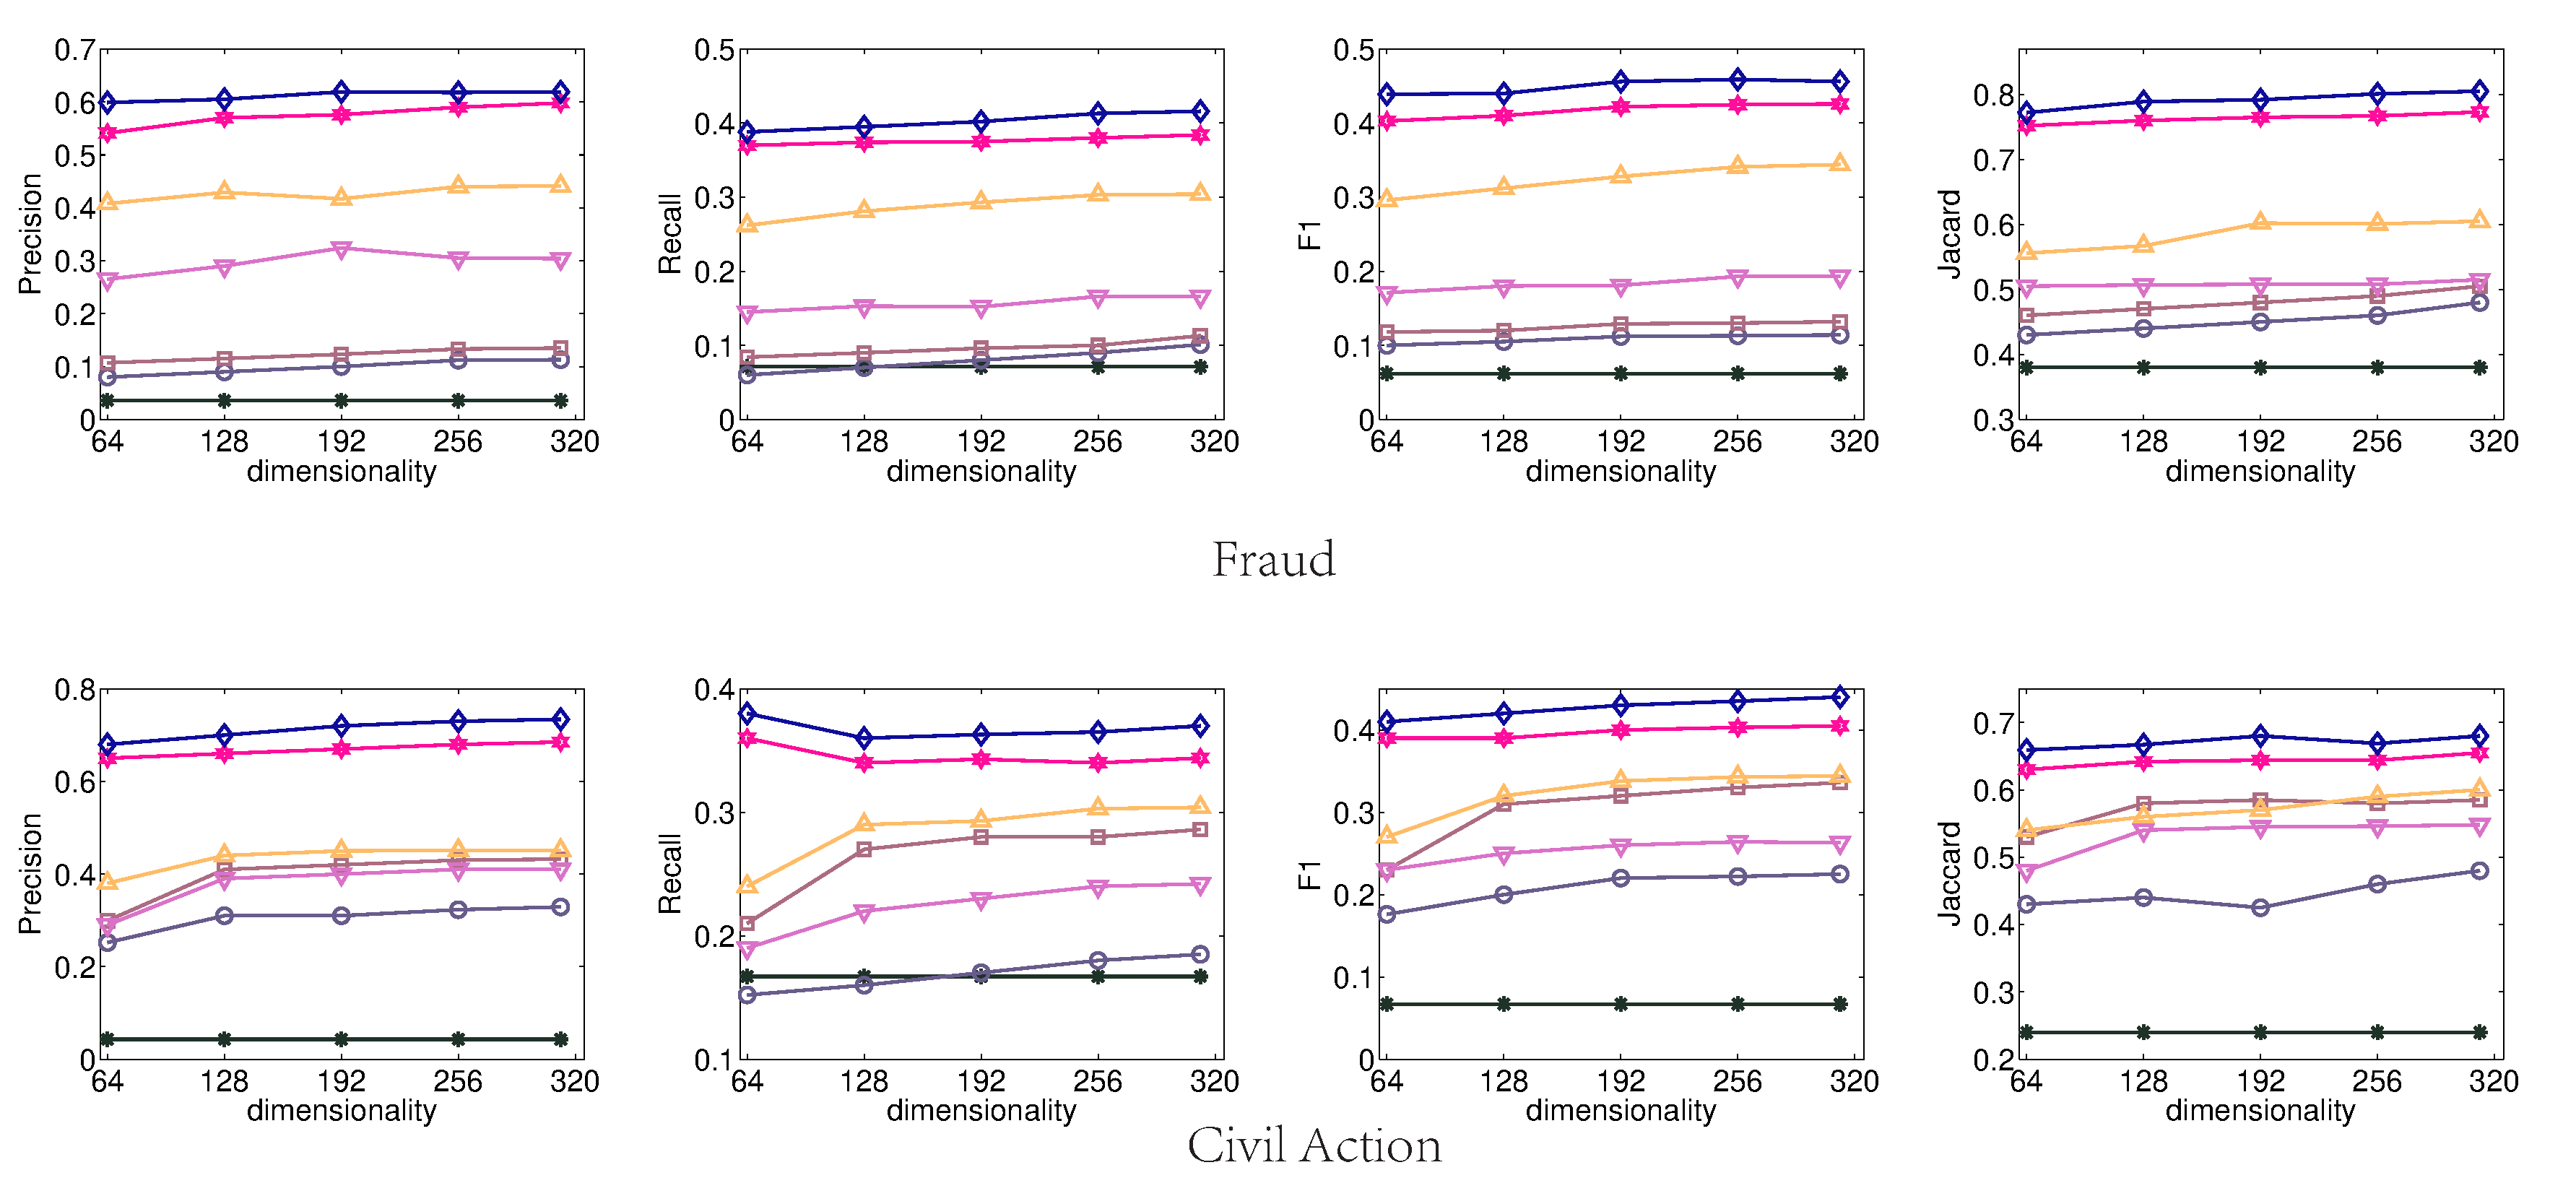
\includegraphics[scale=0.25, clip=true]{./sources/dpam_comMain.eps}
\caption{\label{fig:comMain}DPAM与基线模型实验对比图}
\end{figure*}

该实验中特征维度设置从64到320不等,从实验结果中有以下发现:
\begin{itemize}
    \item 1) 毫不惊讶POP在所有模型中的结果最差,这体现了判决预测是一项不容易的工作。这是由于司法领域标签集合的分布是不规则的,因此对不同的样本预测相同的标签是不恰当的。
    \item 2)一阶方法(BSVM,ML-KNN)的结果好于POP方法。
    \item 3)二阶方法的结果要好于一阶方法,这证明了建模标签关联信息可以有效提升模型性能。以诈骗案由数据集为例,BP-MLL方法相比BSVM方法,在320维特征下Macro-F1上性能提升了$24.4\%$。
    \item 4)TEXTCNN-MLL结果好于BP-MLL,它体现了通过深度神经网络模型可以比浅层模型得到更好的结果。这个结果与之前研究者的发现一致\cite{Kim14}。
    \item 5)CC结果好于BSVM,但是性能提升有限。这个原因是因为,作为链式方法,CC容易受到误差传播的影响\cite{KubatSD10}。例如,当一个分类器误分类了一个像本,错误标签信息将会被传递到下一个分类器。
    \item 6)最后,当利用多任务方式同时学习阈值预测器和多标签分类,DPAM在所有指标上获得了最好的结果。例如,与第二名的方法(TEXTCNN-MLL)进行对比,在Macro-P,Macro-R,Macro-F1和Jaccard的结果分别提升了$2.5\%$, $4.3\%$, $3.5\%$ and $2.0\%$,结果提升明显。
\end{itemize}

\section{分析与讨论}
\label{sec:dpam_analysis}
\subsection{训练策略的影响}
为了学习提出的DPA模型,本课题利用burn-in方法进行优化。该方法中参数$n_{burn}$需要进行设置。本课题对$n_{burn}$的影响进行挖掘研究。

具体地,本课题在诈骗案由数据集上尝试了$n_{burn}\in \{0,200,400,600,800,1000,1200\}$。图~\ref{fig:comS}展示了在特征维度为320时不同burn-in值情况下Macro-F1的结果。
\begin{figure}[htb]%[htbp]
\vspace{-10pt}
\centering
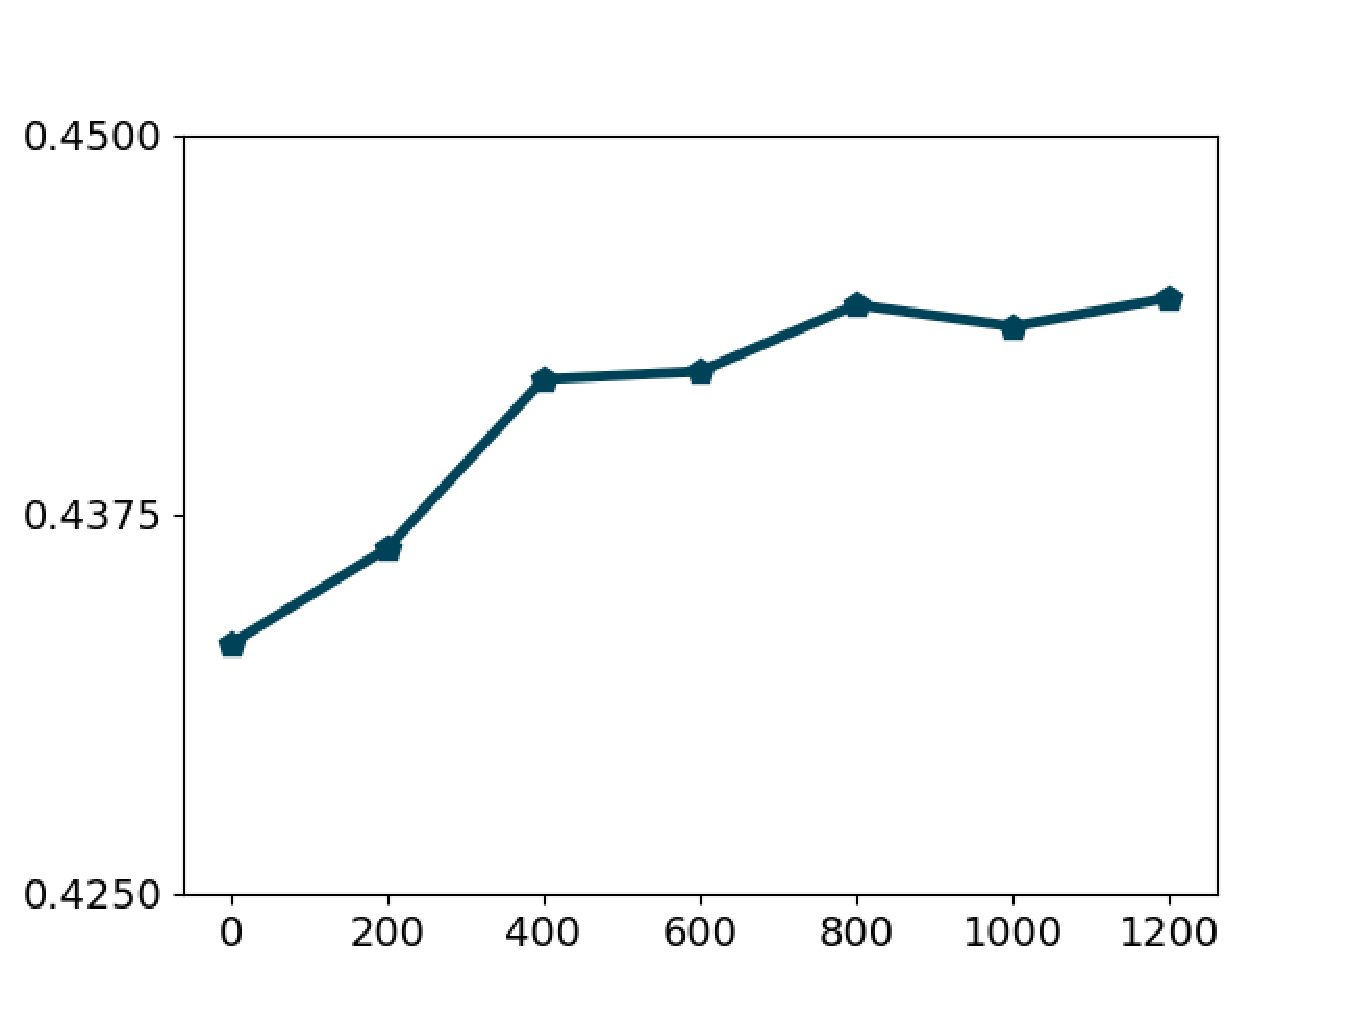
\includegraphics[scale=0.5, clip=true]{./sources/dpam_comS.eps}
\vspace{-20pt}
\caption{\label{fig:comS} 不同burn-in大小影响实验结果图}
\vspace{-10pt}
\end{figure}

该实验中burn-in大小由0到1200不断增加,从实验结果中,可以得到以下结论:
\begin{itemize}
    \item 随着$n_{burn}$不断增大,Macro-F1的结果同时提升。
    \item 当$n_{burn}$的值持续增大,两次不同值下的性能差异越来越小。例如,当$n_{burn}$ 从800增加到1000时,Macro-F1上的相对性能提升由0.3\%。它表示在800词迭代之后,已经获得了相对稳定的词特征表达,如果继续增加迭代次数,继续提升性能变得更困难。因此,在本模型的对比实验中,将$n_{burn}$ 设置为1000。
\end{itemize}

\subsection{案例分析}
为了更好地理解为什么DPAM可以比其他模型获得更好的性能,在本章节中,本课题进行案例分析,比较DPAM和第二名的模型TEXT-CNN的性能。以诈骗案由数据集为例,首先根据出现次数将70个标签进行排序,之后将数据按标签分成7组,每组包含10个标签。通过这种方式,第一组数据包含了出现次数最多的10个标签,最后一组包含了最稀疏的10个标签。给定这个条件,本课题比较了在第一组数据上的模型性能,进行6次重复实验,每次添加下一组数据进行比较。通过这种方式,本课题希望测试当面对标签不均衡问题时,DPAM是否有效。结果展示如图~\ref{fig:comL}:

\begin{figure*}[htbp]%[ht]
\centering
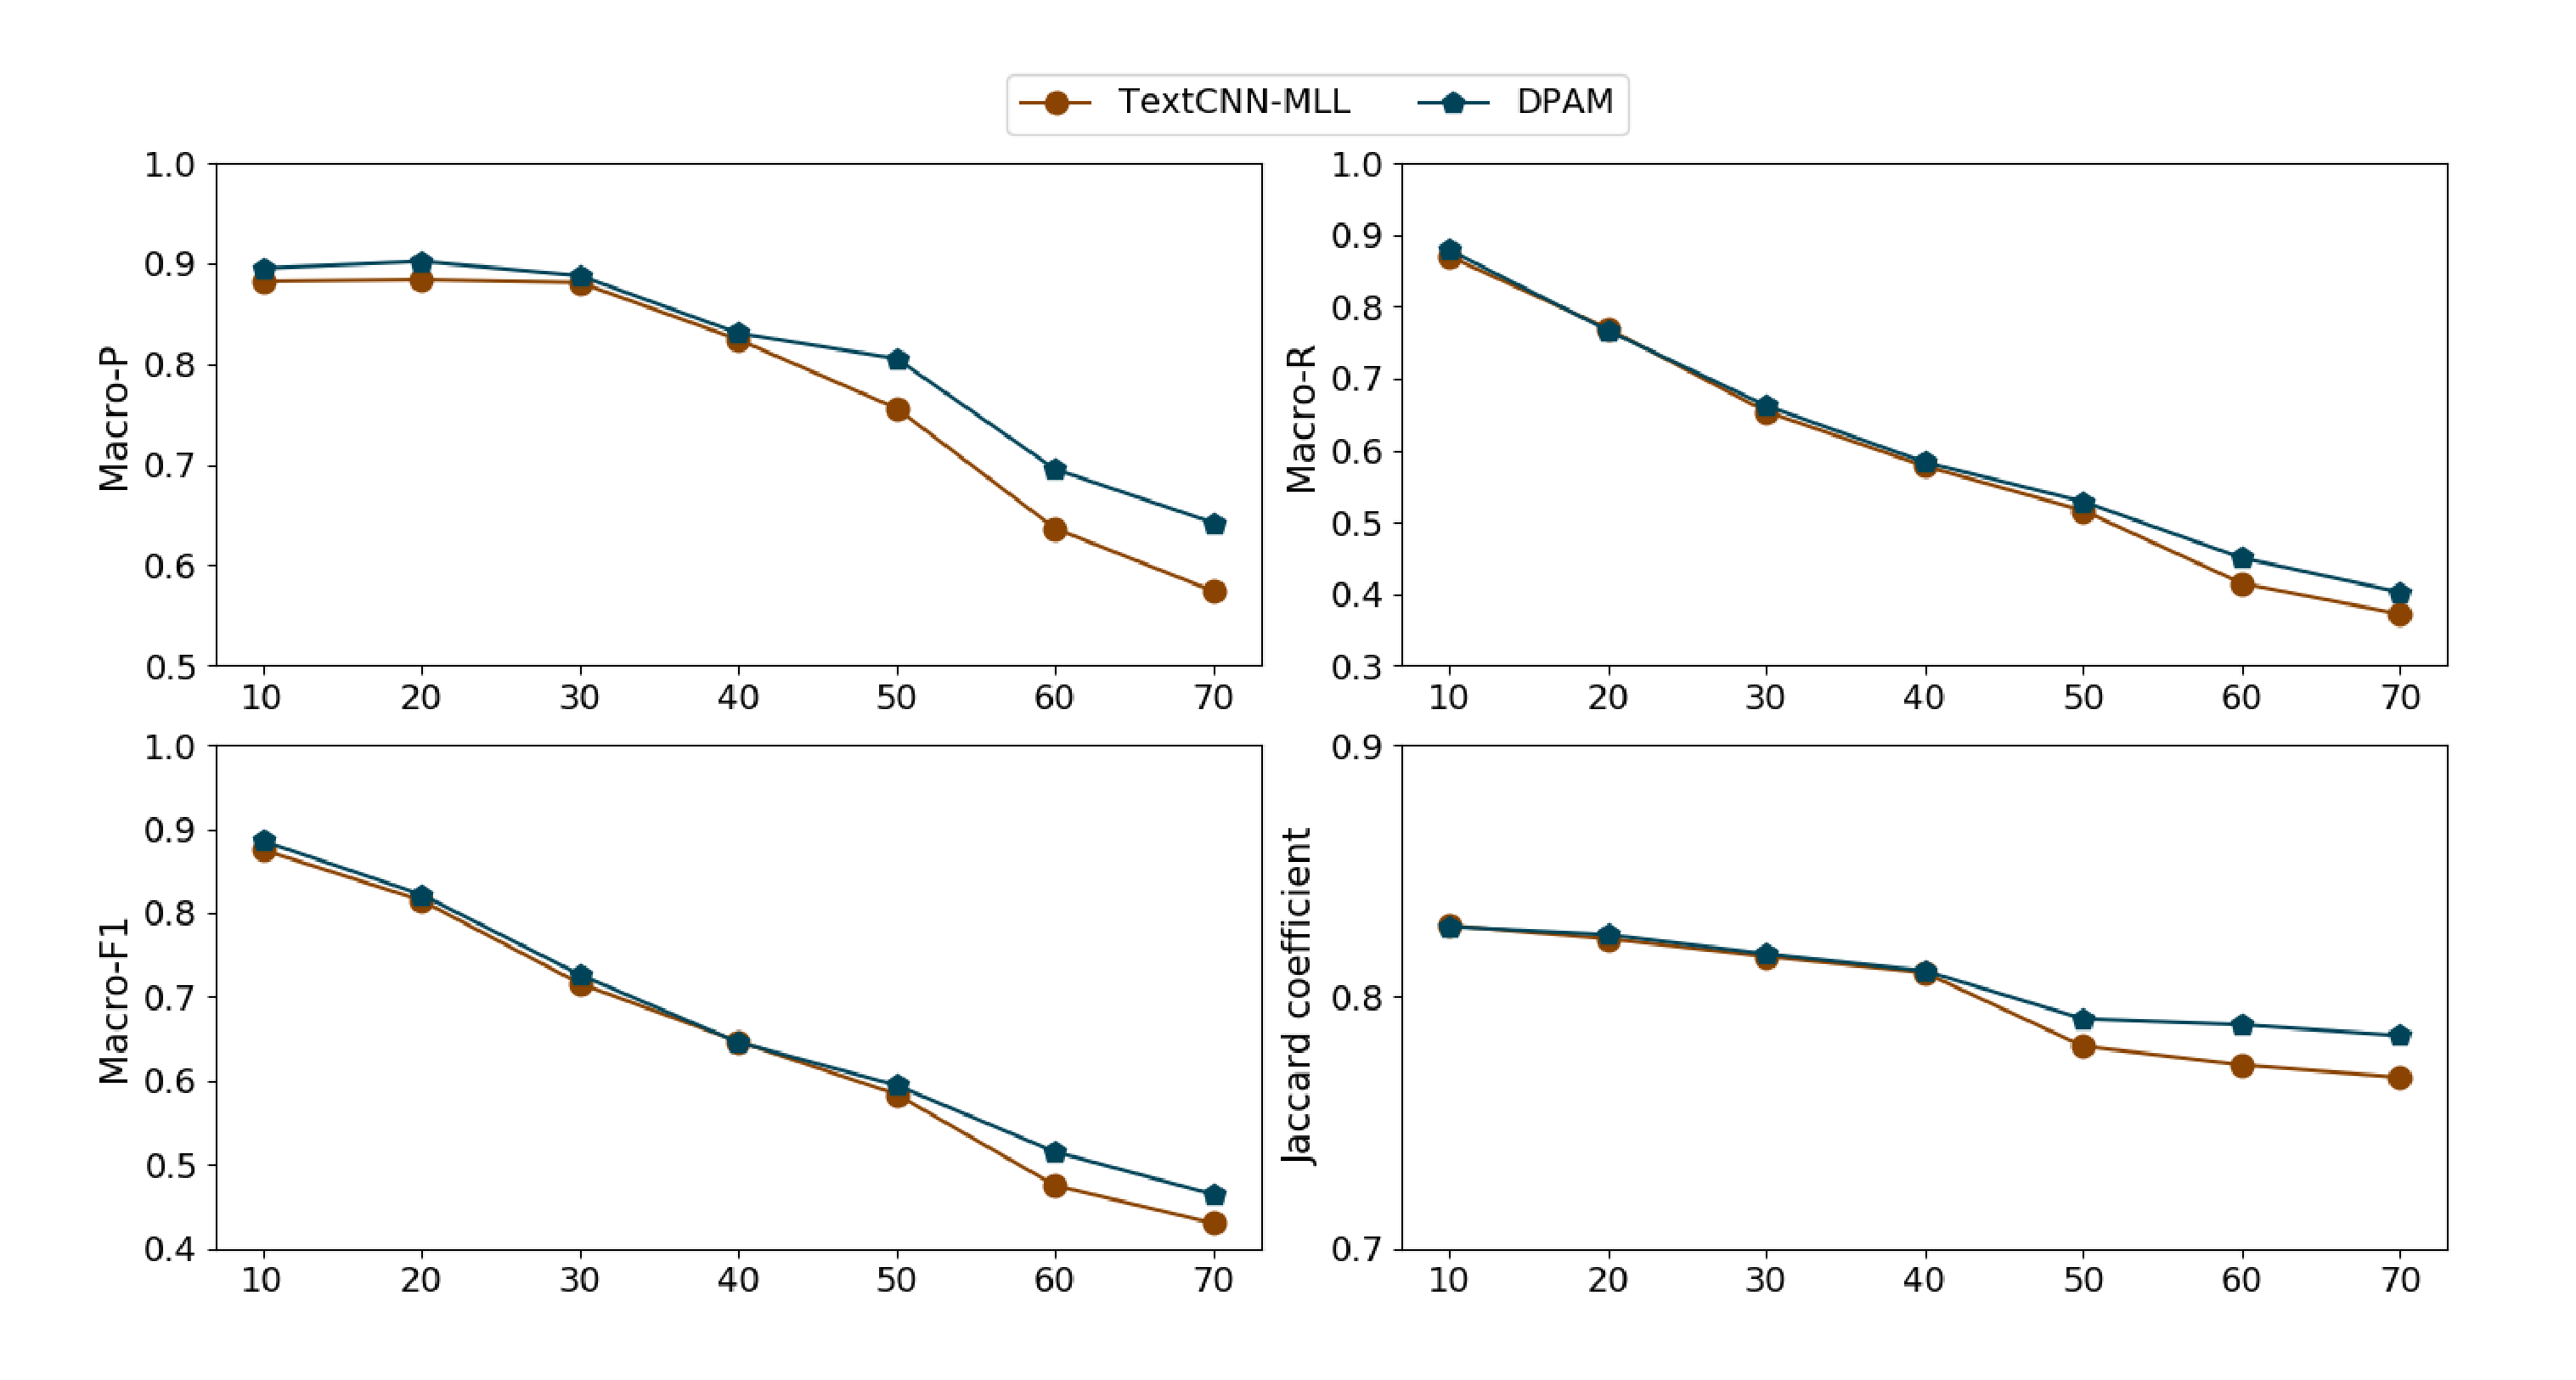
\includegraphics[scale=0.30, clip=true]{./sources/dpam_comL.eps}
\caption{\label{fig:comL}不同标签集合分组实验图}
\end{figure*}

其中x轴代表代表标签集合大小,y轴代表不同指标下的模型性能,从实验结果中,可以有以下发现:
\begin{itemize}
    \item DPAM和TEXTCNN-MLL的结果在考虑更多标签时下降,这与期望的结果一致,当考虑更稀疏的标签,会导致模型结果的降低。
    \item DPAM在添加到第5组数据时,指标全面超越TEXTCNN-MLL。一个有趣的现象是,当之后添加更多组数据时,性能差距越来越大。这意味着DPAM通过引入注意力机制矩阵可以缓解标签不均衡问题。
\end{itemize}

\section{本章小结}
\label{sec:dpam_conclu}
在本章节中,本课题将司法判决预测问题看作多标签分类问题,提出一种动态成对注意力机制的模型(简称DPAM)用来进行法条预测。通过引入从标签定义中学到的注意力机制矩阵,本模型可以缓解标签不均衡问题。本课题之后提出一个动态阈值预测器用来自动学习一个鲁棒的阈值。最后本课题采用多任务框架同时学习多标签分类和阈值预测器,通过利用不同任务之间的信息传递,可以有效提升模型的泛化性能。通过在两个真实数据上的实验验证,证明本课题的方法比之前的方法在不同的评价指标下有明显的提升。
% \chapterbib
